\section{ТЕСТИРОВАНИЕ И ОПТИМИЗАЦИЯ ПРОИЗВОДИТЕЛЬНОСТИ}

\subsection{Методы и инструменты тестирования}

Перед заключительным этапом проводят тестирование базы данных и ее оптимизацию. На этом этапе производятся проверки корректной и эффективной работы базы данных. Кроме того, выполняются тесты производительности, определяются проблемы с ней и соответственно решение этих проблемы путем оптимизации запросов, индексов и настройки СУБД PostgreSQL.

Для тестирования базы данных можно использовать различные методы и инструменты, такие как:

Существуют различные методы и инструменты для проверки базы данных, включая:

\begin{itemize}
    \item модульное тестирование: это проверка отдельных компонентов базы данных, таких как хранимые процедуры, триггеры, функции и другие;
    \item интеграционное тестирование: это проверка совместной работы базы данных с приложением, которое использует эту базу данных;
    \item нагрузочное тестирование: это проверка производительности базы данных в условиях высокой нагрузки;
    \item тестирование безопасности: это проверка уязвимостей базы данных и соответствия ее требованиям безопасности;
    \item ручное тестирование: это проверка базы данных на соответствие требованиям и наличие ошибок, которую выполняет тестировщик вручную.
\end{itemize}



\subsection{Нагрузочное тестирование и оптимизация производительности}

Нагрузочное тестирование БД в PostgreSQL - это процесс измерения производительности и стабильности базы данных при большой нагрузке. Это необходимо для определения максимального количества пользователей и запросов, которые могут быть обработаны базой данных, без ухудшения ее производительности.

Для проведения нагрузочного тестирования БД в PostgreSQL, необходимо выполнить следующие шаги:

\begin{itemize}
    \item определить сценарии использования БД: определить типы запросов, которые будут отправлены к БД, и количество пользователей, которые будут использовать приложение одновременно;
    \item подготовить тестовые данные: создать тестовые данные, которые будут использоваться при выполнении запросов в тестовом окружении. Важно создать реалистичные тестовые данные, чтобы результаты нагрузочного тестирования были максимально близки к реальной нагрузке;
    \item настроить окружение для нагрузочного тестирования: убедиться, что база данных и приложение настроены правильно, чтобы обеспечить максимальную производительность и стабильность;
    \item запустить нагрузочное тестирование: выполнить тестовые сценарии использования БД в тестовом окружении и измерить производительность базы данных, используя метрики, такие как скорость ответа, время выполнения запросов, количество ошибок и использование ресурсов;
    \item анализ результатов: проанализировать результаты нагрузочного тестирования, чтобы определить максимальную нагрузку, которую может выдержать база данных, и определить узкие места, которые могут быть оптимизированы.
\end{itemize}

При тестировании в PostgreSQL можно использовать специальные инструменты, такие как pgbench и Apache JMeter, чтобы автоматизировать процесс выполнения тестовых сценариев и сбора метрик производительности. Важно понимать, что результаты нагрузочного тестирования могут изменяться в зависимости от настроек и конфигурации сервера и базы данных, поэтому рекомендуется проводить тестирование на реальном оборудовании, которое будет использоваться в итоговой среде.

\begin{itemize}
    \item pgbench: это инструмент, входящий в стандартный комплект поставки PostgreSQL. Он предназначен для проведения нагрузочного тестирования на уровне SQL-запросов \cite{online10};
    \item pgBadger: это инструмент для анализа логов PostgreSQL. Он позволяет анализировать логи запросов и генерировать отчеты о производительности базы данных;
    \item HammerDB: это инструмент для тестирования производительности баз данных. Он поддерживает PostgreSQL и позволяет тестировать производительность базы данных на различных уровнях нагрузки;
    \item Sysbench: это инструмент, который может быть использован для тестирования производительности базы данных PostgreSQL. Он позволяет тестировать производительность базы данных на уровне SQL-запросов и многопоточности.
\end{itemize}

Важно помнить, что результаты нагрузочного тестирования БД PostgreSQL могут зависеть от конкретной конфигурации сервера и структуры данных, а также от условий использования базы данных в реальном мире. Поэтому результаты тестирования должны быть интерпретированы с осторожностью и использованы для оптимизации конкретной базы данных.

Оптимизация производительности базы данных PostgreSQL может включать в себя ряд мероприятий, чтобы ускорить выполнение SQL запросов и обеспечить более эффективную работу БД. Вот основные подходы, которые можно эффективно использовать для оптимизации БД PostgreSQL \cite{online8, online9}:

\begin{itemize}
    \item создание правильных индексов: индексы ускоряют выполнение запросов, позволяя PostgreSQL быстро находить нужные данные. Убедитесь, что у вас есть индексы на часто используемые столбцы в запросах, а также на столбцы, используемые в условиях WHERE и JOIN и фильтрации данных, может значительно ускорить выполнение запросов;
    \item оптимизация запросов: оптимизация запросов, такая как использование подзапросов, объединения и группировки данных, может улучшить производительность запросов и уменьшить количество запросов, необходимых для выполнения операции;
    \item разделение данных на отдельные таблицы: если у нас есть большие таблицы, то не следует хранить большие объемы данных в одной таблице. Разделение этих данных на отдельные таблицы или партицирование может помочь ускорить выполнение запросов. Это позволяет более эффективно управлять объемом данных, используемых при выполнении запросов;
    \item оптимизация схемы базы данных: иногда изменение структуры базы данных может привести к улучшению производительности. Например, использование более эффективных типов данных, уменьшение количества NULL значений или устранение избыточных таблиц и связей;
    \item использование кэширования: если важна скорость выполнения, то можно использовать кэширование для часто запрашиваемых данных. Использование кэширования запросов может значительно улучшить производительность, позволяя избежать выполнения сложных запросов, возвращая результаты из кэша. Это особенно полезно для запросов, которые выполняются часто и имеют статические результаты;
    \item оптимизация запросов на запись: если есть интенсивная нагрузка на запись данных, то различные техники, такие как пакетная вставка (batch insert), использование транзакций и пакетных обновлений, могут помочь ускорить процесс записи данных;
    \item предварительная компиляция запросов: в PostgreSQL есть возможность предварительной компиляции запросов (prepared statements), что позволяет повторно использовать выполненные запросы и сократить накладные расходы на компиляцию. Предварительную компиляцию стоит использовать для запросов, которые выполняются многократно с различными параметрами;
    \item настройка конфигурации PostgreSQL: немаловажное значение имеет изучение и настройка параметров конфигурации PostgreSQL в соответствии с требованиями конкретной системы. Некоторые параметры, которые можно настроить, включают размер буферов, параллелизм выполнения запросов и максимальное количество одновременных соединений;
    \item обновление до последней версии PostgreSQL: немаловажное значение имеет актуальность поддерживаемого ПО, поэтому рекомендуется использовать последнюю стабильную версию PostgreSQL. Каждое новое обновление может содержать оптимизации и улучшения производительности, которые могут существенно повысить скорость выполнения запросов;
    \item настройка памяти и дискового пространства: правильная настройка памяти и дискового пространства может существенно повлиять на производительность PostgreSQL. Следует выделять достаточное количество памяти для работы с базой данных. Кроме того, система должна иметь достаточное дисковое пространство для хранения данных и временных файлов;
    \item использование материализованных представлений: материализованные представления - это предварительно вычисленные результаты запросов, сохраняемые в виде таблиц. Они могут быть особенно полезны, если имеются сложные запросы с большими объемами данных, которые выполняются часто. Материализованные представления позволяют значительно сократить время выполнения запросов;
    \item настройка параллелизма: PostgreSQL поддерживает параллельное выполнение запросов, что может значительно ускорить обработку больших объемов данных. Можно настроить параметры параллелизма в зависимости от характеристик системы и требований к производительности;
    \item горизонтальное масштабирование: если даже после оптимизации базы данных путем проведения вышеперечисленных манипуляций все еще возникают проблемы с производительностью , можно рассмотреть вариант горизонтального масштабирования. Распределение данных на несколько серверов может помочь справиться с высокой нагрузкой и улучшить производительность;
    \item оптимизация настройки сервера: настройка параметров сервера PostgreSQL, таких как размер буфера и количество параллельных запросов, может улучшить производительность базы данных.
\end{itemize}

Важно проводить тестирование на реалистичных тестовых данных и сценариях использования, чтобы получить наиболее точные результаты. Также при проведении нагрузочного тестирования БД PostgreSQL необходимо учитывать следующие факторы:

\begin{itemize}
    \item объем данных: чем больше объем данных в базе данных, тем больше ресурсов требуется для обработки запросов. Поэтому важно учитывать объем данных при выборе конфигурации сервера и оптимизации производительности;
    \item конфигурация сервера: настройка сервера PostgreSQL имеет большое значение для производительности базы данных. Например, увеличение размера буфера может ускорить выполнение запросов, но при этом может потребовать больше памяти;
    \item структура данных: структура таблиц и связей между ними может влиять на производительность базы данных. Например, использование ненормализованных таблиц может привести к медленной работе базы данных;
    \item распределение запросов: распределение запросов между разными серверами или узлами может увеличить производительность и снизить нагрузку на базу данных,
\end{itemize}

С учётом вышеперечисленных возможностей для оптимизации и тестирования, было проведено нагрузочное тестирование полностью готовой, оптимизированной и заполненной реальными данными БД для полноценного функционирования web-приложения onmp.ru с помощью модуля PostgreSQL - pgbench.

Для проведения нагрузочного тестирования требуется:

\begin{itemize}
    \item инициализировать базу данных с помощью pgbench. Это создаст необходимые таблицы и заполнит их тестовыми данными:

    «pgbench -i -s 100 database\_name».

    Флаг -s 100 указывает на размер масштабируемости данных, где 100 означает, что будет создано в 100 раз больше строк, чем количество таблиц. Можно изменить это значение в соответствии с потребностями в тестировании;
    \item запускаем нагрузочное тестирование с помощью pgbench. Ниже приведен пример команды, которая запускает тест с 10 параллельными клиентами и общим числом транзакций 1000:
    
    «pgbench -c 10 -j 10 -t 1000 database\_name».
    
    Флаг -c 10 указывает на количество параллельных клиентов, -j 10 указывает на количество параллельных потоков (обычно выбирают такое же значение, как и -c), а -t 1000 указывает на общее количество транзакций для выполнения;
    \item далее анализируем результаты тестирования, которые будут выведены в консоль. Они включают среднее время выполнения транзакции, количество транзакций в секунду и другие метрики производительности;
    \item затем будем просто изменять параметры команды pgbench, такие как количество клиентов, количество потоков и общее количество транзакций, чтобы провести более интенсивное или длительное тестирование.
\end{itemize}

С подробными результатами нагрузочного тестирования можно ознакомиться в приложении Б. По полученным результатам можно увидеть и смело сделать вывод, что разработанная база данных в полной мере выдерживает нагрузки при больших объемах хранимых и обрабатываемых данных. Кроме того, при одновременном подключении порядка 50-80 пользователей, система выдержала нагрузку и задержка на подключение пользователя к сессии составляет всего около 0.5 секунд, что никак отрицательно не отражается на работоспособности и корректном функционировании web-приложения.

Тестирование БД PostgreSQL является важным этапом при разработке и оптимизации базы данных. Оно позволяет выявить узкие места в работе базы данных и произвести необходимую оптимизацию, чтобы обеспечить максимальную производительность и стабильность приложения.

Стоит отметить, что после внедрения базы данных необходимо проводить анализ ее использования и результата. Это позволит выявить потенциальные улучшения и оптимизации процессов работы с медицинской информацией. На основе анализа можно внести изменения в структуру базы данных, внедрить новые функциональные возможности или улучшить существующие.



\subsection{Выполнение запросов}

После того, как мы разобрались с видами тестирования, оптимизацией памяти и скорости выполнения запросов, самое время продемонстрировать полученные результаты.

На рисунке~\ref{fig:fig21} представлен SQL запрос к таблицам медикаментов, представленных на рисунке~\ref{fig:fig07}.

\begin{figure}
  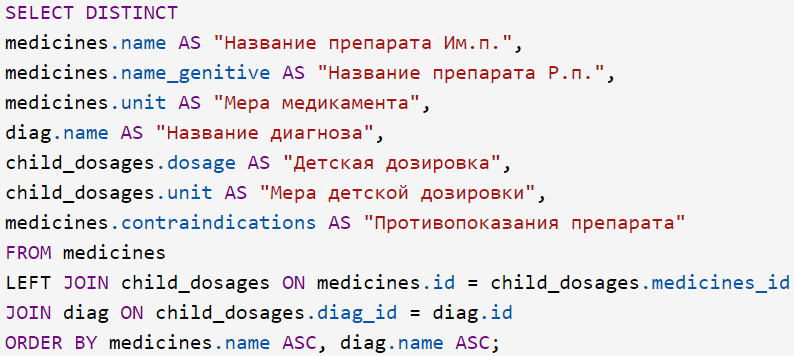
\includegraphics[scale=0.78]{inc/sh_all_ch_med}
  \caption{SQL запрос получения всех медикаментов}
  \label{fig:fig21}
\end{figure}

Запрос есть, теперь нужно посмотреть корректность выводимых данных. На рисунке~\ref{fig:fig22} представлен вывод SQL запроса с рисунка~\ref{fig:fig21}.

\begin{figure}
  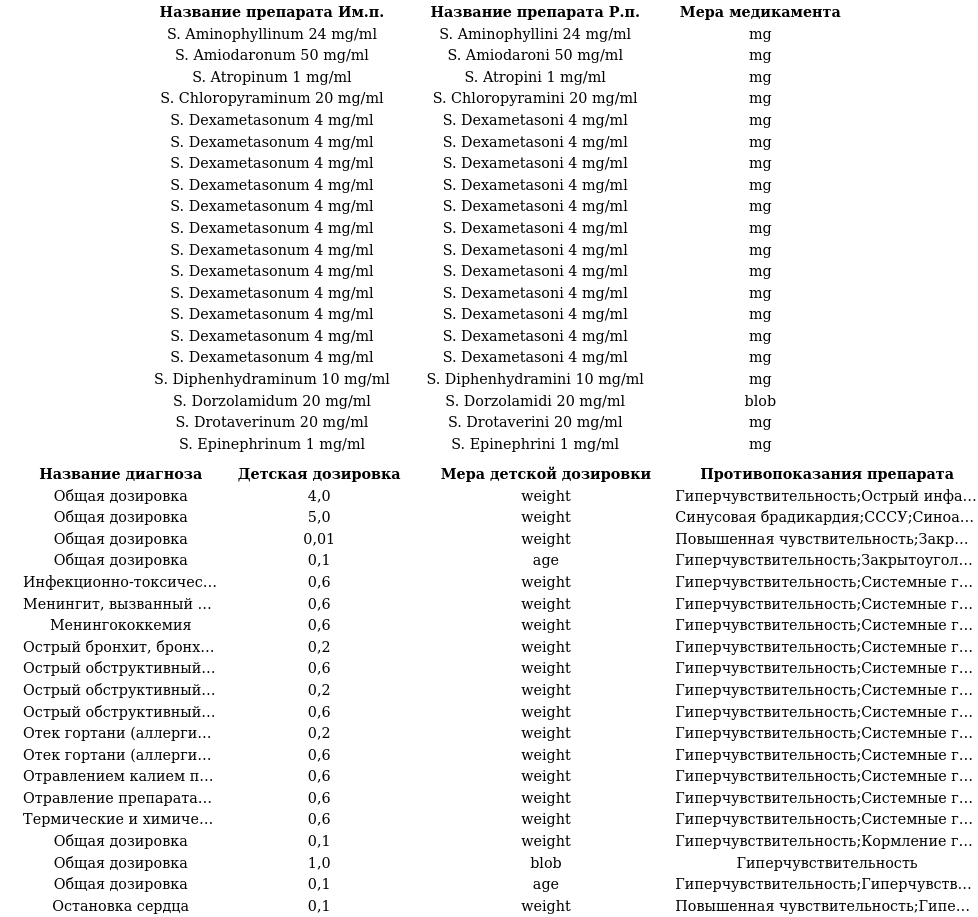
\includegraphics[scale=0.955]{inc/sh_all_ch_med1}
  \caption{Результаты запроса к таблицам медикаментов}
  \label{fig:fig22}
\end{figure}

Все результаты моей деятельности - проектирования, выполнения запросов и их оптимизация, впоследствии передаются на бэкенд. На рисунке~\ref{fig:fig23} представлен JSON формат по отображению всех медикаментов со взрослыми и детскими дозировками из данных, полученных при обращении к БД.

\begin{figure}
  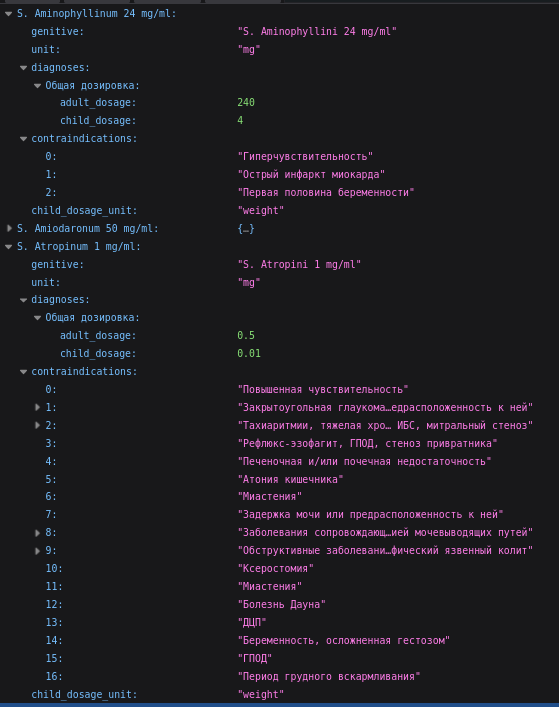
\includegraphics[scale=1.1]{inc/json_sh_all_med1}
  \caption{JSON формат данных, полученных при обращении бэкенда к таблицам медикаментов}
  \label{fig:fig23}
\end{figure}

На рисунке~\ref{fig:fig24} представлен SQL запрос к таблицам заболеваний, представленных на рисунке~\ref{fig:fig06}.

\begin{figure}
  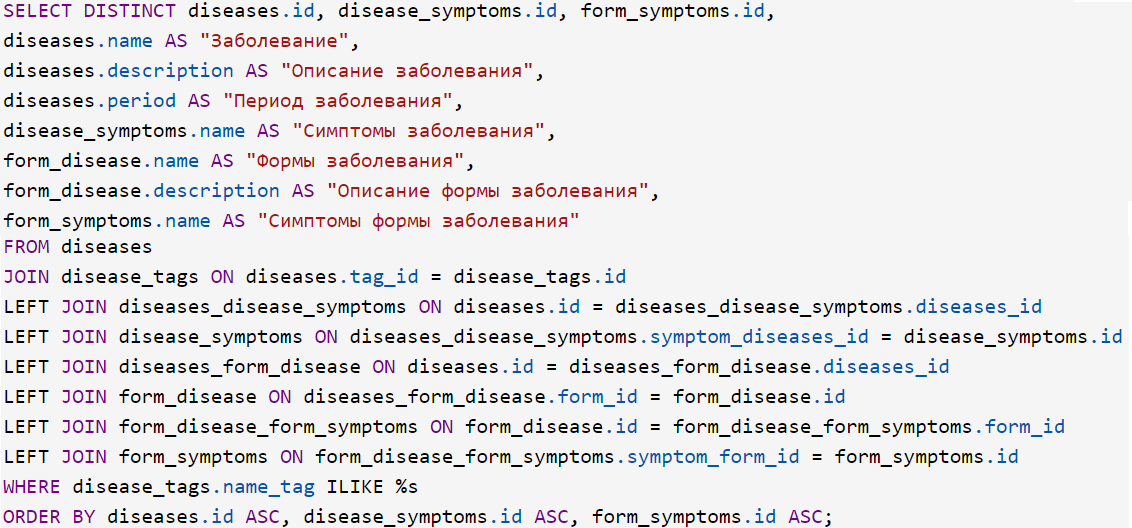
\includegraphics[scale=0.82]{inc/json_sh_dis_part_name}
  \caption{SQL запрос по части названия заболевания}
  \label{fig:fig24}
\end{figure}

На рисунке~\ref{fig:fig25} представлен вывод SQL запроса с рисунка~\ref{fig:fig24}.

\begin{figure}
  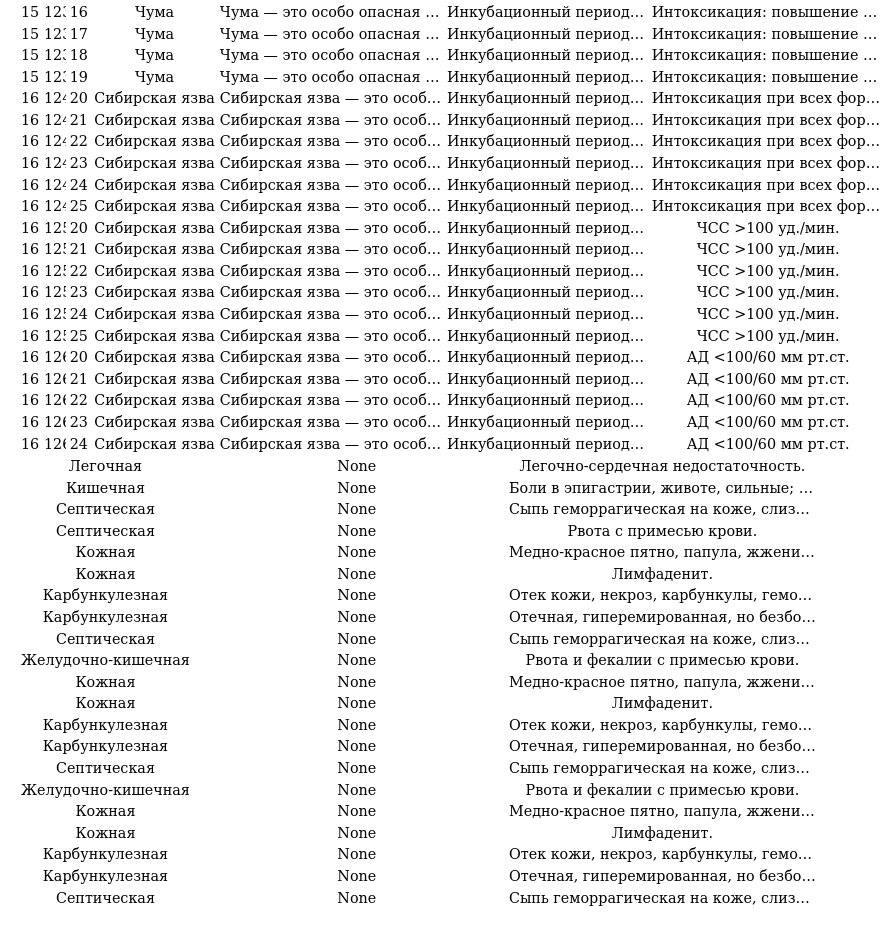
\includegraphics[scale=0.87]{inc/json_sh_dis_part_name1}
  \caption{Результаты запроса к таблицам заболеваний}
  \label{fig:fig25}
\end{figure}

На рисунке~\ref{fig:fig26} представлен JSON формат по отображению всех заболеваний из данных, полученных при обращении к БД.

\begin{figure}
  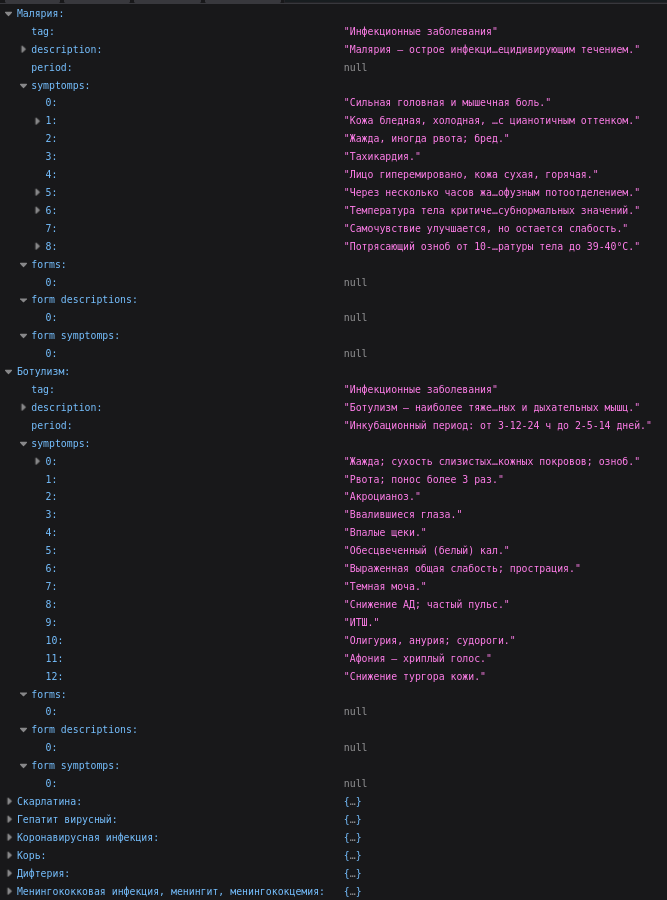
\includegraphics[scale=0.92]{inc/json_sh_dis_part_name2}
  \caption{JSON формат данных, полученных при обращении бэкенда к таблицам заболеваний}
  \label{fig:fig26}
\end{figure}

На рисунках выше были приведены примеры запросов и полученные данные основных таблиц: заболевания, диагнозы и медикаменты. Но кроме основных, еще имеются вспомогательные таблицы дифференциальной диагностики, которые носят информативно-вспомогательный характер.

На рисунке~\ref{fig:fig27} представлены SQL запросы к таблицам дифференциальной диагностики для корректного взаимодействия с бэкендом.

\begin{figure}
  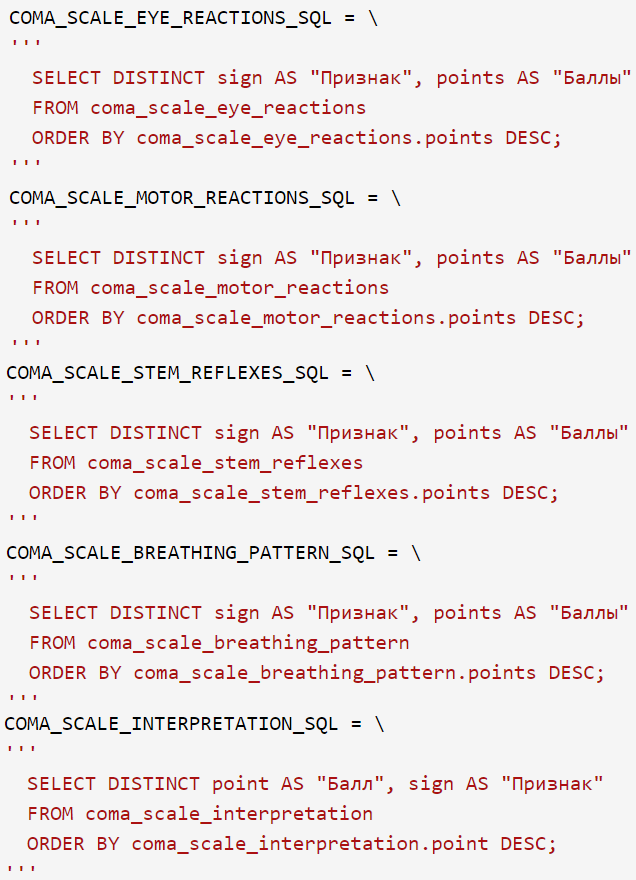
\includegraphics[scale=1.1]{inc/sh_one_table}
  \caption{SQL запросы к таблицам дифференциальной диагностики}
  \label{fig:fig27}
\end{figure}

На рисунке~\ref{fig:fig28} представлен JSON формат таблиц дифференциальной диагностики из данных, полученных при обращении бэкенда к БД.

\begin{figure}
  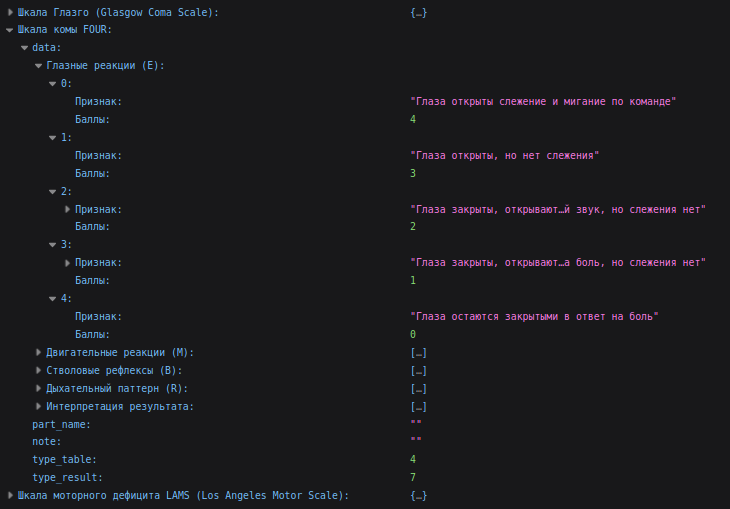
\includegraphics[scale=0.83]{inc/sh_one_table1}
  \caption{JSON формат данных, полученных при обращении к таблицам заболеваний}
  \label{fig:fig28}
\end{figure}

На рисунке~\ref{fig:fig29} представлен JSON формат всех таблиц дифференциальной диагностики.

\begin{figure}
  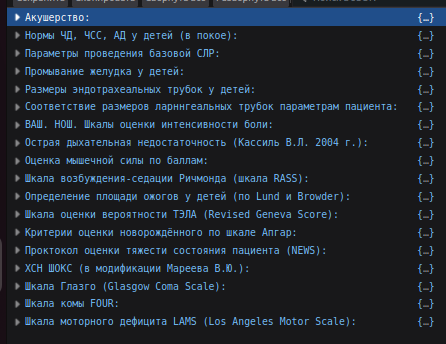
\includegraphics[scale=1]{inc/sh_all_tables}
  \caption{Таблицы дифференциальной диагностики}
  \label{fig:fig29}
\end{figure}



\bigbreak
\textbf{Выводы по разделу}
\bigbreak

Тестирование базы данных является критически важным этапом в разработке и поддержке приложений, использующих базы данных. Тестирование базы данных позволяет убедиться в корректности и надежности ее работы, а также обеспечить защиту от ошибок и нарушений безопасности.

Использование различных методов и инструментов позволяет выявить проблемы в базе данных еще на ранних стадиях и устранить их до того, как они приведут к серьезным проблемам в работе приложения. Кроме того, тестирование базы данных помогает повысить уровень доверия пользователей к приложению и защитить данные от нарушений и утечек. В целом, проведение тестирования базы данных является критически важным для обеспечения надежности, безопасности и производительности приложений.